\documentclass{llncs}
\usepackage[show]{ed}
\usepackage{wrapfig}
\usepackage{xspace}
\usepackage{graphicx}
\usepackage{stex-logo}
%\usepackage{lststex} debug that the gray is not solid
\usepackage{listings}
\definecolor{codegray}{rgb}{0.9,0.9,0.9}
\lstset{basicstyle=\sf,columns=fullflexible,backgroundcolor = \color{codegray}}
\lstset{numberstyle=\tiny}
\lstset{language={[LaTeX]TeX}}
\usepackage[style=alphabetic,hyperref=auto,defernumbers=true,backend=bibtex,firstinits=true,maxbibnames=9,maxcitenames=3,isbn=false]{biblatex}
\addbibresource{kwarcpubs.bib}
\addbibresource{extpubs.bib}
\addbibresource{kwarccrossrefs.bib}
\addbibresource{extcrossrefs.bib}
\usepackage[noabbrev]{cleveref}

% I do not want to annotate just yet.

\newcommand\ALeA{\textsf{ALeA}\xspace}
\newcommand\snify{\textsf{snify}\xspace}
\def\llangle{\langle\kern-.2em\langle}
\def\rrangle{\rangle\kern-.2em\rangle}

\title{Bulk Semantic Annotation with a Partially Known Knowledge Base}
\author{Michael Kohlhase, Jan Frederik Schaefer}
\institute{Computer Science, FAU Erlangen N\"urnberg, Germany}
\begin{document}
\maketitle
\begin{abstract}
tbw
\end{abstract}

\section{Introduction}
Arguably, dealing with large document collections is one of the key factors in the
knowledge-driven society and economy. There are currently two main contenders for machine
support in this area. Symbolic/logic-based technologies and sub-symbolic,
machine-learning-based AI, e.g.\ via LLMs or chatbots. They have complementary strengths
and challenges: Symbolic technologies offer precision and explainability out of the box,
but face scalability challenges because the prerequisite background knowledge has to be
(manually) formalized. ML-based approaches can be trained on all data of the Internet, but
face challenges in precision and explainability. In \cite{Ranta:atcp17},
Aarne Ranta matches these profiles to the notion of \textbf{producer tasks} -- i.e.\ tasks
where precision is key, but limited coverage ($10^{3\pm1}$ concepts) is OK;
e.g.\ for multi-language/variant manuals for very
expensive machines -- and \textbf{consumer tasks}, where coverage is key and
precision secondary; e.g.\ for consumer-grade machine translation like \textsf{Google translate}.

In this paper, we address tools that help attack the coverage problem in symbolic/semantic
approaches in practice. The producer task we use as a case study is that of adaptive
learning assistants for MINT subjects, concretely the \ALeA system \cite{BerBetChu:lssmkm23}.
\ALeA uses \sTeX \cite{MueKo:sdstex22,sTeX:github:on} -- a
variant of {\LaTeX} that allows to embed semantic annotations -- for knowledge
representation, and generates learner-adaptive learning objects instrumented with
learning-support interactions from that. The \textbf{\sTeX/\ALeA content commons}
\ednote{MK@MK: continue to describe the size and distribution, and
  authorship}\ednote{explain the \textbf{domain model} (the SMGloM) and the
  \textbf{formulation model} (cf. \cite{BerBetChu:lssmkm23}) in the commons and give their
  relative sizes.}

We contend that while education -- especially higher education -- as a whole is a
wide-coverage task for society education of individual learners in specific domains --
especially, if we want to tailor the educational offerings to said individual/domain -- is
a producer task, at least until ML-based methods reach the precision and explainability
required by the ethics of teaching.

\section{Semantic Authoring in a Content Common}
The main practical problem of annotating presentational {\LaTeX} course materials into
semantic documents that carry enough information to support meaningful learning support
services is to add semantic references to technical terms from the domain jargon. Take for
instance a learning object like the paragraph in \cref{fig:lo}, where we want to annotate
the the term ``terminal'' with the (semantic) concept of ``a goal state of a search problem''. The latter can either be defined earlier in the course or in the domain model
(or both).

\begin{figure}[ht]\centering
  \fbox{\includegraphics[width=10cm]{../example2.pdf}}
  \caption{An annotated Learning Object from an AI Lecture}\label{fig:lo}
\end{figure}

Concretely this is about converting the {\LaTeX} string
\begin{lstlisting}[numbers=left,firstnumber=3,
caption=The {\LaTeX} sources of \cref{fig:lo},label=lst:los]
\item \blue{Note:} Depth-limited minimax requires an evaluation for every
cut-off state $s$. If $s$ is terminal, we use its utility, and otherwise
an estimate.
\end{lstlisting}
into the (partially) annotated item:
\begin{lstlisting}[morekeywords={sr,importmodule},numbers=left,
caption=Annotating ``terminal'' in \cref{lst:los},label=lst:losa]
\importmodule[smglom/search]{mod?search-problem}
[...]
\item \blue{Note:} Depth-limited minimax requires an evaluation for every
cut-off state $s$. If $s$ is \sr{goal state}{terminal}, we use its utility,
and otherwise an estimate.
\end{lstlisting}
% Concretely, the author has to remember the module that introduces the concept
% of terminal states (\cref{fig:state-space}),
% the symbol name \lstinline|goal state|, annotate it with the
% \sTeX macro \lstinline[mathescape]|\sr{$\llangle symbol name \rrangle$}{$\llangle verbalization\rrangle$}|, and add the module import in the first line (unless it
% is already imported).
% If the symbol name and the desired verbalization coincide,
% the short-hand macro \lstinline|\sn| can be used (e.g. \lstinline|\sn{utility}|).

% In this case the symbol name happens to be the same as its English
% verbalization, otherwise we would have to use
% \lstinline[mathescape]|\sr{$\llangle symbol name\rrangle$}{state space}|.
The annotation is legitimized\ednote{grounded?} by a definition in the domain model module shown in
\cref{fig:state-space}. The \lstinline|\definame| in line 3 introduces the
\textbf{verbalizations} ``goal state'' and ``terminal state''
for the symbol \lstinline|search-problem?goal state|
introduced be \lstinline|\symdecl*| declaration in line 3.

\begin{figure}[ht]\centering
  \fbox{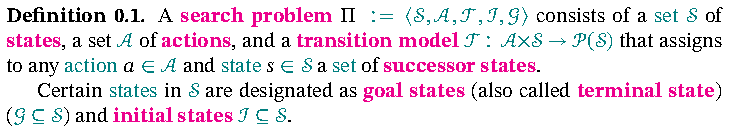
\includegraphics[width=12cm]{../search-problem.en.pdf}}
\begin{lstlisting}[morekeywords={definame,symdecl},numbers=left]
\begin{smodule}[title=Search Problem]{search-problem}
[... some imports ...]
\symdecl*{goal state}
\begin{sdefinition}
  [...] Certain \sns{state} are [...] \definame[post=s]{goal state} [...]
  (also called \definiendum{goal state}{terminal states}).
\end{sdefinition}
\end{smodule}
\end{lstlisting}
  \caption{Simplified definition of ``goal state'' from the domain model}\label{fig:state-space}
\end{figure}

To annotate the string ``terminal'' in the learning object,
the author has to be aware that it is a technical term,
that the module from \cref{fig:state-space} exists, know the
symbol name and its URL\ednote{path?}, and manage redundancy of the imports -- i.e. only adding the
\lstinline|\importmodule| directive if it is not already (recursively) implied and
possibly removing directives that become redundant by the new one.
At ca 150,000 words in
a semester's words of lecture notes and ca. 10--15\%\ednote{can we actually measure this for AI?} of technical terms a rather daunting
task.

\sTeX authoring is already supported by an VSCode IDE plugin \cite{sTeX-IDE:git} that
analyzes annotations on the fly, displays the underlying reference semantics, reports
errors and redundancies, and even offers a concept search interface. But these only offer
support already for annotated terms, so they do not solve the annotation problem above.

\section{The \snify System}

The \snify system (see \cite{stextools:git}) is a simple command-line tool that creates a
database of symbol-verbalization pairs, analyzes \sTeX source files and then steps through
all word occurrences in the document that share the stem with a verbalization in the
database. For each such word, the user is presented with an annotation choice and
interactions that allow to fine-tune the wordwise annotation workflow. \Cref{fig:snify}
shows a typical situation.\ednote{MK: I like the example less and less! We need an example
  that has at least one homostem (another verbalization that has the same stem; introduce
  the concept her and use it throughout) so that we can show the choice mechanism, and
  where the verbalization is different from the symbol name. Having a two-word compound is
  good though.} 

\begin{figure}[ht]
  \fbox{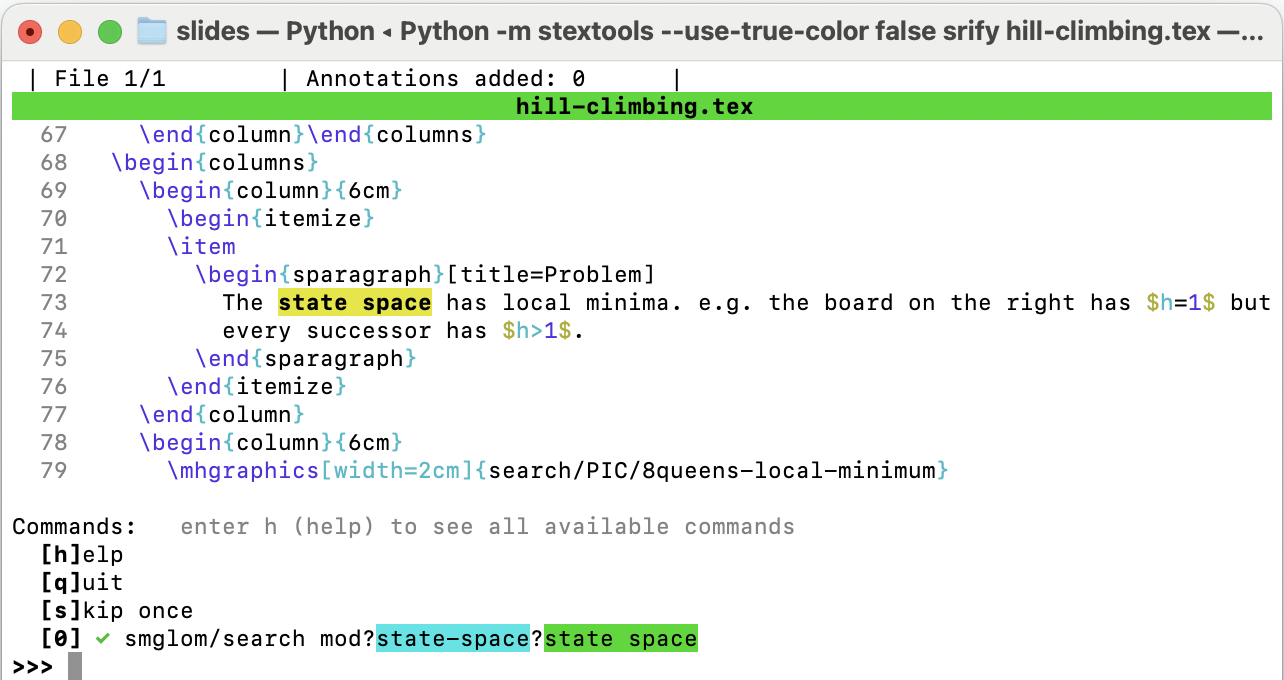
\includegraphics[width=12cm]{../img/srify}}
  \caption{\snify in Action: Annotating the term ``state space''.}\label{fig:snify}
\end{figure}

Here the annotator can choose an annotation by typing the corresponding choice
number. Here, the module \lstinline|state-space| is already imported (see the little green
check-mark); otherwise \snify would offer the annotator the choice to import it -- if we are
in a module context -- or to add a \lstinline|\usemodule| directive and where (in the
local environment or top-level). Alternatively, typing \lstinline|s| skips this word,
\lstinline|S| skips and adds a comment to always skip this word, and -- if \snify first
suggests the term `state` \lstinline|n| extends it to the compound ``state space'' by
including the next word.

\snify is usually called on a set of files -- e.g. in a directory or math archive -- which
together form a \textbf{session}, which can be interrupted and resumed without having to
re-do all the \lstinline|s| skips. Alternatively, \snify can be called e.g. on the top-level
lecture notes; then the session consists of all included files. Other productivity
features include a focus mode that can be used to propagate a particular choice to the
rest of the file, session, or the whole \sTeX/\ALeA corpus before resuming regular
annotation This reduces the cognitive effort from choosing a symbol from a list to
deciding whether a particular choice is applicable in the current document context. Of
course the include management still needs to be done locally.

\section{Practical Evaluation}

In our experience, the step-through workflow for annotating term references for symbols
from the domain model is almost an order of magnitude more efficient than writing the
annotations and imports by hand, even for annotators who are familiar with the domain
model. For annotators unfamiliar with the domain model, the unassisted annotation task is
almost infeasible, and the average unfamiliarity naturally grows with the domain
model. The symbol disambiguation process -- on average a word induces $n$\ednote{MK@FS: we
  should try to measure this: for every verbalization (i.e. symbol/word pair) we should
  compute the ratio of those words with the same stem.} choices is still manageable,
requires considerable concentration and domain knowledge, but little knowledge of the
domain model flexiformalization.

The command-line interface is simple and responsive and gives all the necessary
information in a single glance if underlying shell area exceeds ca. $80\times 35$
characters. It is very much geared towards annotating existing documents with respect to a
relatively complete -- pre-existing -- domain model, and it seems unlikely that a more
sophisticated UI would add value for this use-case.

For less complete domain models we have to skip too many terms that should ultimately be
annotated and annotation efficiency suffers. This is currently the case for all
non-English languages in the \sTeX corpus we work with. Coverage in German is only about
half of that of English and we can already see the practical effects. We have also
experimented with a Slovene introductory math book, and it seems clear that apart from
having to introduce a Slovene stemmer\ednote{MK@FS: there is one for python at
  \url{https://repo.ijs.si/pboskoski/slo_stemmer}}, we would need to manually annotate all
definienda in the book before we can harvest the symbol/verbalization pairs which are a
prerequisite for annotation.

The current interface is not well-suited for on-the-fly annotation while editing while
authoring. For that, the underlying information (the symbol/verbalization pairs harvested
from the domain model) can be integrated into any IDE. In fact we plan to do this for the
next version of the sTeX plugin for VSCode \cite{sTeX-IDE:git}.

\section{Conclusion}

In this system description we have presented the \snify tool, a command-line tool
\ednote{continue} \snify is open source\ednote{MK@FS: do we have an explicit license yet in
  the repository.}; the source and documentation are available from \cite{stextools:git}.

In an earlier attempt to support semantic annotation in IDEs, we tried named-entity
recognition (NER) for classification of ``likely annotation candidate words''
\cite{hutterer:msc23}, however this classification was not precise enough in the
distinction in ``technical terms'' and ordinary English noun phrases and named entities --
the relevant task for annotation, and so made it impractical, especially, since it could
not enter the actual annotations and import directives automatically. But maybe using the
NER-based approach, after the \snify annotation process might change the trade-offs
involved. In any case, the overall workflow suggested by the NER-based approach --
especially after the verbalizations covered by the existing domain model\ednote{introduce
  in the definition above that the domain model is all definitions, not only in the
  smglom?} -- is geared towards adding modules and symbols -- the ones discovered by NER
-- to the domain model. 



\printbibliography
\end{document}

%%% Local Variables:
%%% mode: latex
%%% TeX-master: t
%%% End:

% LocalWords:  tbw Aarne Ranta homostem pre
